\section{Results}\label{sec:Results}

\subsection{Mortgage Classifier (Benchmark)}\label{subsec:Mortgage Classifier (Benchmark) Results}

In order to assess whether a predictive algorithm would pick up on and reproduce bias in the data, an initial classification model (as described in \textbf{chapter \ref{subsec:Model_Training_and_Prediction}} and detailed in \textbf{table \ref{tab:CH03_Model_Details}}) was trained on the HMDA dataset (see \textbf{chapter \ref{subsec:HMDA_Data}}) with the goal of predicting whether a mortgage would be granted or not for a given applicant.
The results of this model were assessed in terms of performance and fairness as described in \textbf{chapter \ref{subsec:Performance_Assessment}} and \textbf{chapter \ref{subsec:Fairness_Assessment}}, respectively.

\textbf{Performance Assessment}

When fitting the neural network to the training data, the \textit{training accuracy} of the model improved rapidly initially, leveling off after a few epochs. The \textit{validation accuracy} started at a high level and constantly improved by small increments, suggesting that both the model learning process as well as the ability to generalize to previously unseen data were successful. 
The training process was stopped by an early\_stopping callback, with the ninth epoch being the one with the least validation loss. The training results of the best epoch were:
\begin{itemize}
    \item \textit{Training Accuracy}: 0.90
    \item \textit{Validation Accuracy}: 0.90
    \item \textit{Training Loss}: 0.28
    \item \textit{Validation Loss}: 0.28
\end{itemize}
The history of the training process is depicted in \textbf{figure \ref{fig:Model_Training_History}}.

\begin{figure}
    \centering
    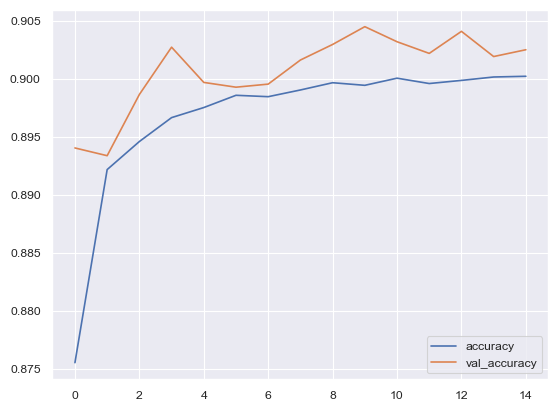
\includegraphics[width=0.85\textwidth]{images/Model_Training/Initial_Training_History.png}
    \caption{Training History of the Mortgage Classifier Model}
    \medskip
    \small
    The training history of the initial mortgage classifier model, showing the training and validation accuracy and loss over the course of the training process. The training accuracy improved constantly until the early\_stopping callback. The validation accuracy constantly improved, suggesting a successful learning process.
    \label{fig:Model_Training_History}
\end{figure}

The model was then evaluated on the test dataset, which was not seen by the model during training. The results of the performance evaluation (i.e. \textit{metrics \#1}) are shown in \textbf{table \ref{tab:Model_Evaluation}}. The model achieved an \textit{accuracy} of 0.90, a \textit{precision} of 0.88, a \textit{recall} of 0.97, and an \textit{F1-score} of 0.92. 
As stated in \textbf{chapter\ref{subsec:Performance_Assessment}}, the original model output were probabilities between 0 and 1. These could be used to calculate ROC AUC and plot the corresponding ROC curve, which can be seen in \textbf{figure \ref{fig:Model_Training_ROC}}. The \textit{ROC-AUC} score was 0.94, indicating a high level of model performance. 
Converting the probabilities into predictions with a threshold of 0.5 fulfilled the classification requirement. The \textit{confusion matrix} is depicted in \textbf{figure \ref{fig:Model_Confusion_Matrix}}. The model managed to achieve a high number of true positives and true negatives, while the number of false negatives was low. However, the number of false positives was nearly 8\% of all predictions.

\begin{table}[h]
    \centering
    \begin{tabular}{l c}
    \toprule
    \textbf{Metric} & \textbf{Value} \\
    \midrule
    \textbf{accuracy} & 0.90 \\
    \textbf{precision} & 0.88 \\
    \textbf{recall} & 0.97 \\
    \textbf{f1} & 0.92 \\
    \bottomrule
    \end{tabular}
    \caption{Metrics \#1: Initial Model}
    \small
    The mortgage classifier model was evaluated on the test dataset, achieving an accuracy of 0.90, a precision of 0.88, a recall of 0.97, and an F1-score of 0.92.
    \label{tab:Model_Evaluation}
\end{table}

\begin{figure}
    \centering
    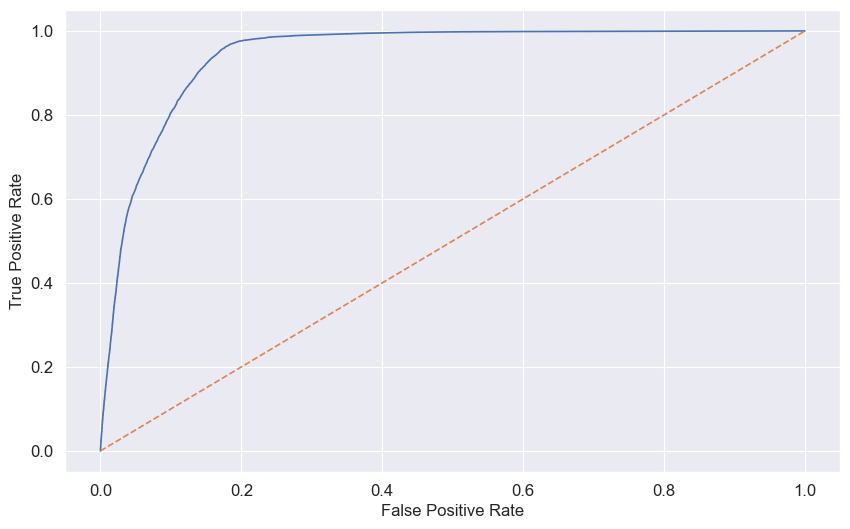
\includegraphics[width=0.85\textwidth]{images/Model_Training/Initial_ROC_curve.png}
    \caption{ROC curve of the Mortgage Classifier Model}
    \medskip
    \small
    The ROC curve is significantly above the diagonal baseline, indicating high predictive performance.
    \label{fig:Model_Training_ROC}
\end{figure}

\begin{figure}
    \centering
    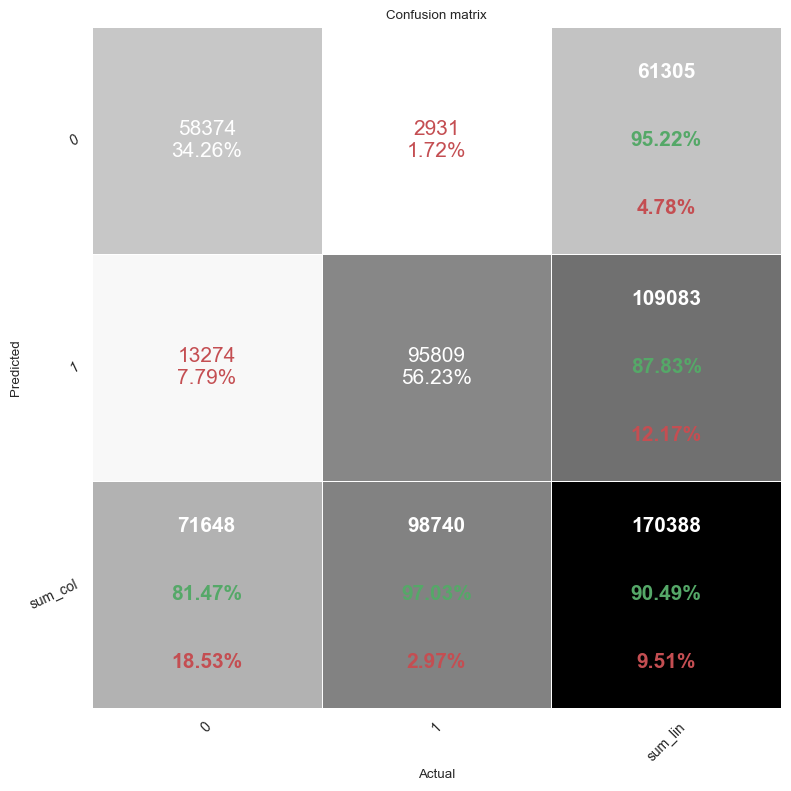
\includegraphics[width=0.85\textwidth]{images/Model_Training/Initial_Confusion_Matrix.png}
    \caption{Confusion Matrix on the Test Dataset of the Mortgage Classifier Model}
    \medskip
    \small
    The confusion matrix of the mortgage classifier model on the test dataset. The model achieved a high number of true positives and true negatives. The number of false negatives was low, however, false positives made up nearly 8\% of all predictions.
    \label{fig:Model_Confusion_Matrix}
\end{figure}

\textbf{Fairness Assessment}

Following the research question (see \textbf{chapter \ref{ch:Introduction}}), the \textit{detection of unfairness} in the predictions is an explicit goal of this thesis. To address this, the fairness assessment outlined in \textbf{chapter \ref{subsec:Fairness_Assessment}} was applied to the predictions. The results of the fairness assessment (i.e. \textit{metrics \#2}) are shown in \textbf{table \ref{tab:Fairness_Assessment_Initial}}. 
The model performed slightly better for \textit{White} applicants than for \textit{Black} applicants. The \textit{accuracy} for \textit{White} applicants was 0.91, while it was 0.88 for \textit{Black} applicants. The \textit{precision} for \textit{White} applicants was 0.89, while it was 0.82 for \textit{Black} applicants. The \textit{recall} for \textit{White} applicants was 0.97, while it was 0.96 for \textit{Black} applicants. 
The \textit{F1-score} for \textit{White} applicants was 0.93, while it was 0.88 for \textit{Black} applicants. The \textit{AUC} for \textit{White} applicants was 0.94, while it was 0.95 for \textit{Black} applicants. 
In terms of disparities (where the optimal value is \textbf{1}), the model performed comparably well in all disciplines except the \textit{fnr\_disparity}, which was 1.42. This indicates that the model was more likely to predict a false negative for \textit{Black} applicants than for \textit{White} applicants.

\begin{table}[h]
    \centering
    \begin{tabular}{lr}
    \toprule
    \textbf{Metric} & \textbf{Value} \\
    \midrule
    \textbf{Accuracy White} & 0.91 \\
    \textbf{Precision White} & 0.89 \\
    \textbf{Recall White} & 0.97 \\
    \textbf{F1 Score White} & 0.93 \\
    \textbf{AUC White} & 0.94 \\
    \midrule
    \textbf{Accuracy Black} & 0.88 \\
    \textbf{Precision Black} & 0.82 \\
    \textbf{Recall Black} & 0.96 \\
    \textbf{F1 Score Black} & 0.88 \\
    \textbf{AUC Black} & 0.95 \\
    \midrule
    \textbf{tpr\_disparity} & 0.99 \\
    \textbf{fpr\_disparity} & 0.96 \\
    \textbf{tnr\_disparity} & 1.01 \\
    \textbf{fnr\_disparity} & 1.42 \\
    \bottomrule
    \end{tabular}
    \caption{Metrics \#2: Initial Model}
    \label{tab:Fairness_Assessment_Initial}
    \small
    The benchmark model showed a slightly better performance for \textit{White} applicants than for \textit{Black} applicants. The disparities were comparably low, except for the \textit{fnr\_disparity}, which was 1.42.
\end{table}

\subsection{Explainability}\label{Explainability Results}

As stated in \textbf{chapter \ref{subsec:Explainability}}, three different approaches to explainability were utilized not only to support the analysis of fairness by providing insights into the model's decision-making process, but also to provide a better understanding of the model's behavior: \textit{SHAP}, \textit{LIME}, and a \textit{Global Surrogate Model}. 

\textbf{SHAP}

XXX

The \textit{expected value} of the SHAP values (i.e. the baseline before consideration of any feature importance) was \textit{0.57}. This corresponds to the imbalance in the original HMDA data (see \textbf{chapter \ref{fig:CHXX_Target_Variable_Distribution}}).

XXX

% Try point summary plot for individual prediction

\textbf{Figure \ref{fig:SHAP_Individual_Analyses}} shows the SHAP values for four selected applicants. The force plots displayed show how the individual values of the features influence the model's decision according to SHAP. 
Each individual prediction results from the aforementioned \textit{expected value} and the sum of inferred importances of the features (exemplarily, in the first plot displayed in \textbf{figure \ref{fig:SHAP_Individual_Analyses}}, the feature importances amount to roughly positive 0.4, leading to a total value of 0.97 and therefore a positive prediction, i.e. a granted mortgage).
It shows that SHAP attributes a high importance to (missingness of) the Debt to income ratio. Due to the values being scaled, a value of \textit{-0.59} corresponds to \textit{debt\_to\_income\_ratio\_missing == False} and a value of \textit{1.68} corresponds to \textit{debt\_to\_income\_ratio\_missing == True}. Therefore, SHAP considers missingness in this variable as negative and availability as positive.
Considering the last applicant displayed (\textit{Black or African American Male, Debt to Income Ratio available}), it does however show that even availabilty of the Debt to Income Ratio does not guarantee a positive model decision.
According to SHAP, none of the decisions displayed here (and in the whole set of predictions in general) were significantly informed by any protected attribute. However, confounding factors might still be present, as the model might have learned to discriminate based on other features that are correlated with the protected attributes.

\begin{figure}[h]
    \centering
    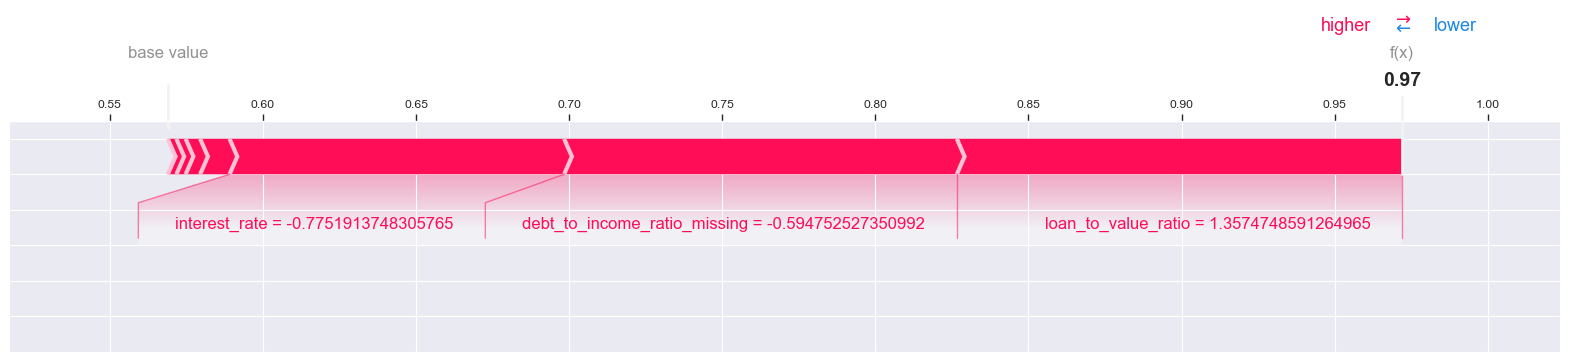
\includegraphics[width=1\textwidth]{images/SHAP_Individual_Analyses/SHAP_individual_0.png}
    \small
    White Male, Debt to Income Ratio available
    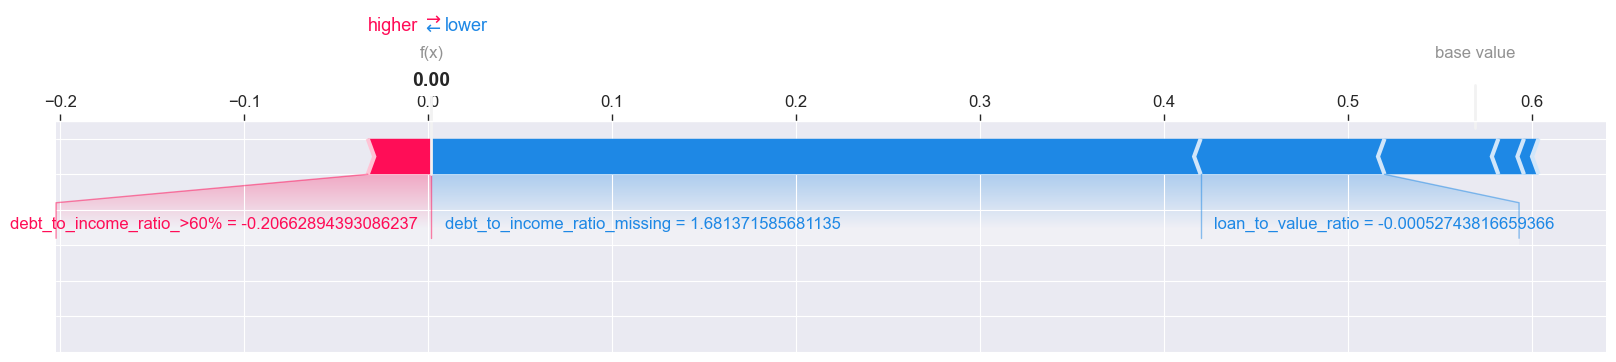
\includegraphics[width=1\textwidth]{images/SHAP_Individual_Analyses/SHAP_individual_1.png}
    \small
    White Male, Debt to Income Ratio missing
    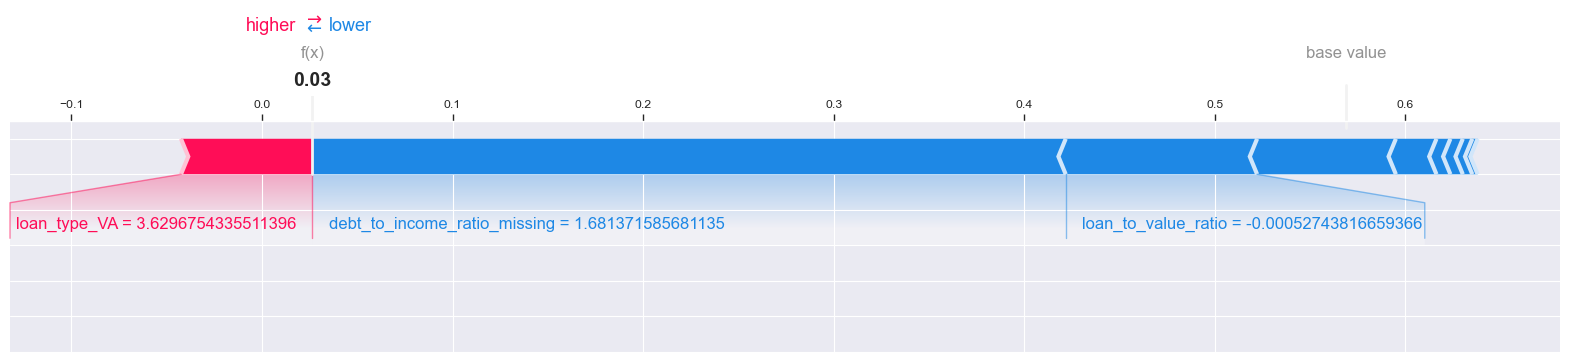
\includegraphics[width=1\textwidth]{images/SHAP_Individual_Analyses/SHAP_individual_21.png}
    \small
    Black or African American Male, Debt to Income Ratio missing
    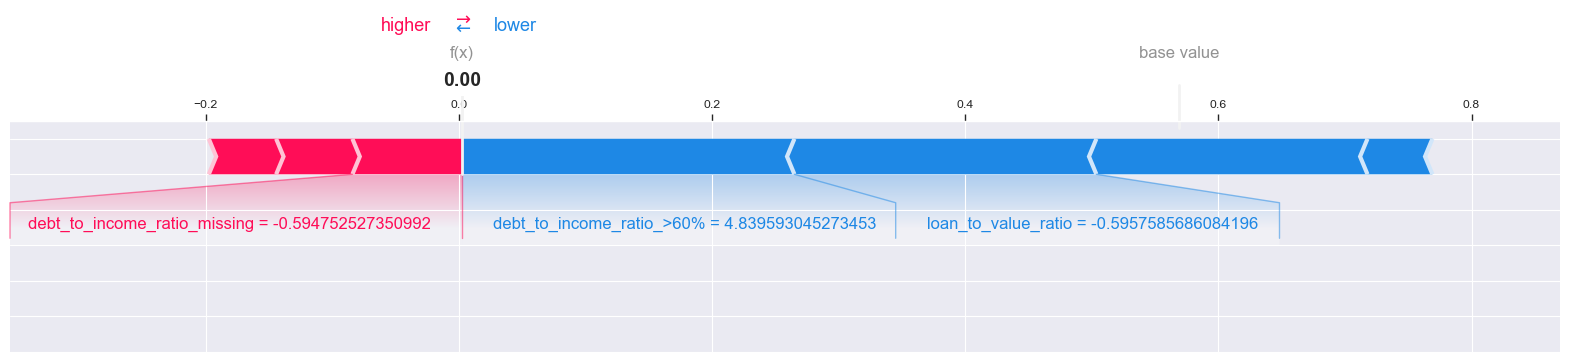
\includegraphics[width=1\textwidth]{images/SHAP_Individual_Analyses/SHAP_individual_139.png}
    \small
    Black or African American Male, Debt to Income Ratio available
    \caption{Selected SHAP Individual Analyses}
    \medskip
    \small
    Comparing four selected Male applicants with different characteristics shows that, in general, SHAP attributes a high importance to (missingness of) the Debt to Income Ratio. However, it is not the sole decision criterion, as the last applicant displayed shows.
    \label{fig:SHAP_Individual_Analyses}
\end{figure}

\textbf{LIME}

XXX

\textbf{Global Surrogate Model}

To validate the results of the local explanations, a \textit{Global Surrogate Model} was used. \textbf{figure \ref{fig:Global_Surrogate}} shows the results of the global surrogate model. Specifically, the five most important features according to the global surrogate model are compared to the SHAP and LIME explanations in terms of their relative performance.
It shows that all three explanation algorithms agree on the three most important features in the data (\textit{debt\_to\_income\_ratio\_missing, interest\_rate}, and \textit{debt\_to\_income\_ratio\_>60\%}), although LIME attributes a different order of importance to them compared to SHAP and the global surrogate model.

\begin{figure}[h]
    \centering
    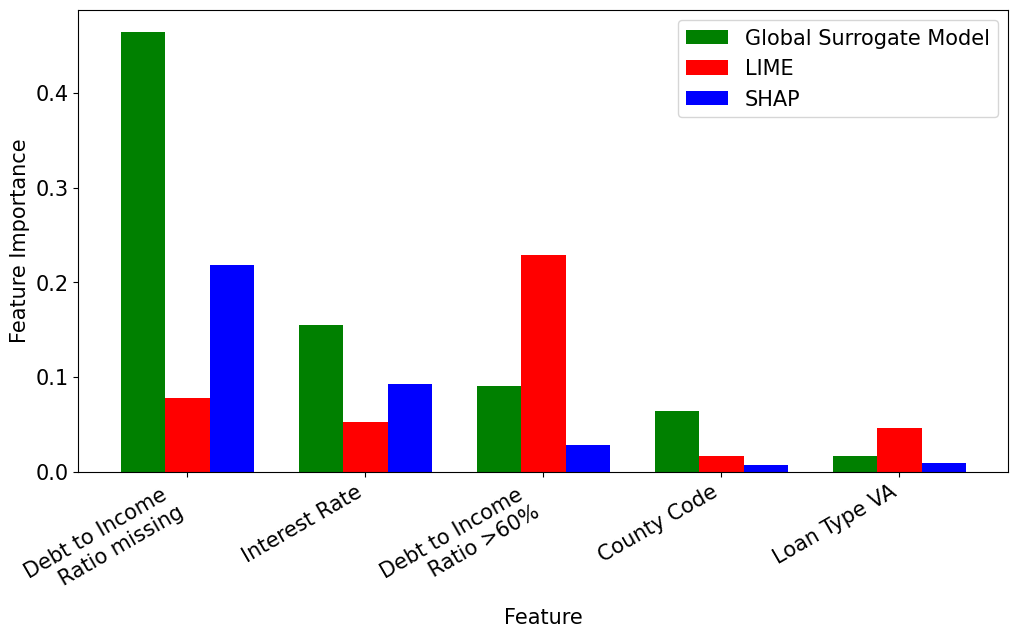
\includegraphics[width=0.85\textwidth]{images/CHXX_UPDATE_Surrogate_SHAP_LIME_combined.png}
    \caption{Global Surrogate Model compared to SHAP and LIME}
    \medskip
    \small
    Analyzing the 5 most important features according to the global surrogate model implies that the overall trends of SHAP and LIME are close to the global explanations.
    \label{fig:Global_Surrogate}
\end{figure}

\subsection{Fairness Adjustments}\label{Fairness Adjustments Results}

While the performance of the benchmark mortgage classifier detailed in \textbf{chapter \ref{subsec:Mortgage Classifier (Benchmark) Results}} was satisfactory, the scope of this thesis (see \textbf{chapter \ref{ch:Introduction}}) included taking an iterative approach to improve fairness without sacrificing predictive performance, as outlined in \textbf{chapter \ref{subsec:Iterations}}.
To this end, the following fairness adjustments were applied to the model: \textit{Reweighing}, \textit{Correlation Remover} and \textit{Calibrated Equalized Odds}. The aim was to reach improvement in at least one of the two metric sets, comapred to the benchmark performance depicted in \textbf{table \ref{tab:Model_Evaluation}} (\textit{metrics \#1}) and \textbf{table \ref{tab:Fairness_Assessment_Initial}} (\textit{metrics \#2}).

\textbf{Reweighing}

XXX

\textbf{Correlation Remover}

XXX

\textbf{Calibrated Equalized Odds}

XXX

\textbf{Summary}

